\chapter{Architectural Views}

\section{Context View}

\subsection{Stakeholders' uses of this view}

\subsection{Context Diagram}

\begin{figure}[H]
    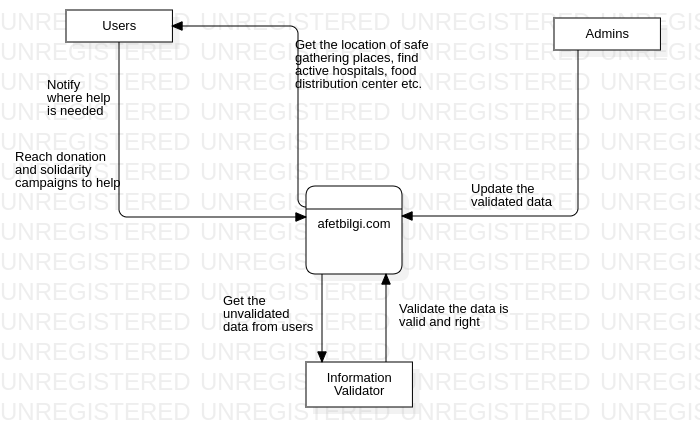
\includegraphics[scale = 0.6]{assets/Context Diagram.png}
    \caption[Context Diagram for afetbilgi.com]{Context Diagram for afetbilgi.com}
\end{figure}

As it can be observed from the context diagram, the system interacts with 3 external entities. These are users, admins and information validators. Afetbilgi.com users can use this website for 2 purpose. It can be used to deliver help or it can be used to get help who are affected by the disaster.
in addition to that, information validator gets the all information which delivered to them and by reaching the authorities validates the information. In meanwhile, admins update the database with these validated datas in the system.

\subsection{External Interfaces}

\subsection{Interaction scenarios}

\section{Functional View}

\subsection{Stakeholders' use of this view}

\subsection{Component Diagram}

\subsection{Internal Interfaces}

\subsection{Interaction Patterns}

\section{Information View}
This view focuses on describing the information requirements Afetbilgi.com. Data operations are examined in this view.

\subsection{Stakeholders' uses of this view}
\begin{itemize}
    \item The volunteers use this view to understand which information they should send while submitting something to website.
    \item The victims use this view to understand what is the meaning of the information they get from website.
    \item The developers use this view to successfully add, edit and delete data from website.
\end{itemize}

\subsection{Database Class Diagram}
\begin{figure}[H]
    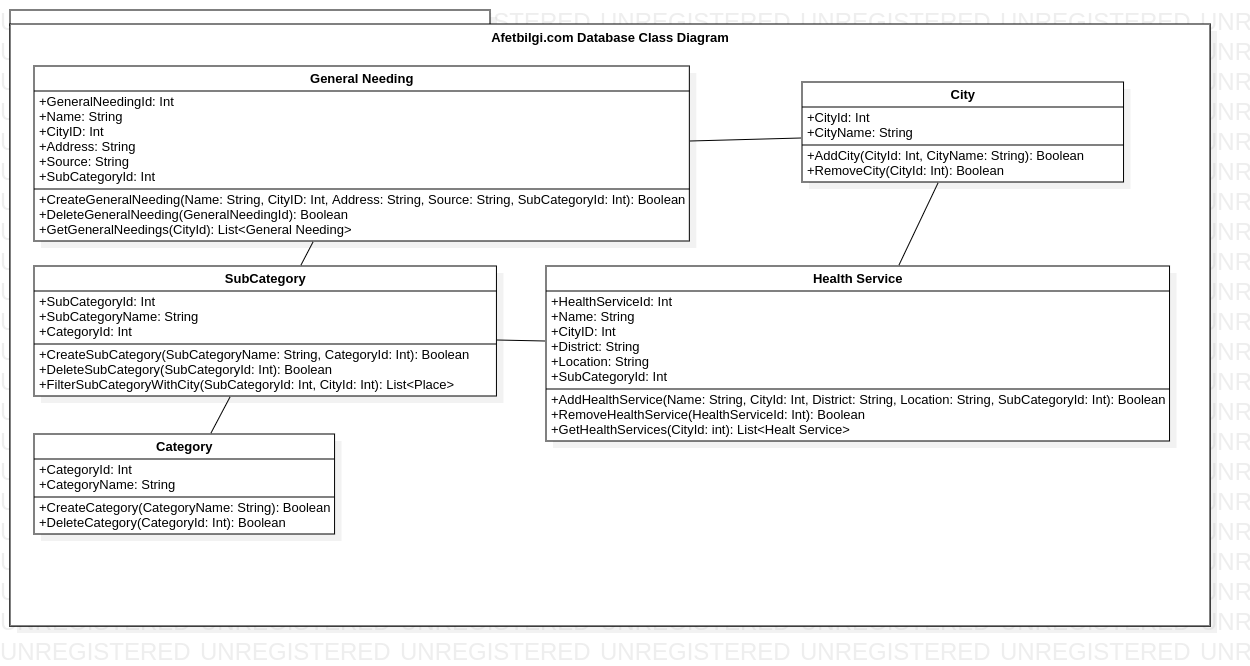
\includegraphics[scale = 0.4]{assets/DatabaseClassDiagram1.png}
    \caption[Database Class Diagram Of Afetbilgi.com]{Database Class Diagram Of Afetbilgi.com}
\end{figure}

\subsection{Operations on Data}
\begin{table}[H]
    \begin{tabular}{|p{6cm}|p{10cm}|}
        \hline
        \textbf{Operation}   & \textbf{Description}                                                                                                                                    \\
        \hline
        \hline
        CreateGeneralNeeding & Crete a new general needing with given attributes returns result.                                                                                                       \\
        \hline
        DeleteGeneralNeeding                & Deletes general needing with given id returns true if successfully deleted.                                                                                                        \\
        \hline
        GetGeneralNeedings                  & Returns a list of general needings in given cityID. \\
        \hline
        CreateCategory                & Creates a category with given name returns success state.                                                                                   \\
        \hline
        DeleteCategory          & Deletes a category and its subcategories returns success state.\\
        \hline
        CreateSubCategory & Creates a subcategory in given category with given name returns result of operation.\\
        \hline
        DeleteSubCategory & Deletes a subcategory with its needings and services returns true if successfully deleted, otherwise returns false.\\
        \hline
        FilterSubCategory & Returns a list of general needings or healthcare services in a city with given subcategory, for example hospitals in Hatay.\\
        \hline
        AddCity & Adds a city with given id and name.\\
        \hline
        RemoveCity & Removes a city with healthcare services and general needings associated with the city.\\
        \hline
        AddHealthService & Adds a new healthcare service with given name, city, district, location and subcategory.\\
        \hline
        RemoveHealthService & Removes the healthcare service with given id.\\
        \hline
        GetHealthServices & Returns healthcare services in a city.\\
        \hline
    \end{tabular}
    \caption[Operations on Data]{Operations on Data}
\end{table}


\section{Deployment View}
This view focuses on how Afetbilgi.com is physically deployed in terms of hardware and software.

\subsection{Stakeholders' uses of this view}
\begin{itemize}
    \item Volunteers can use this view to understand how the system is deployed.
    \item Developers can use this view while updating and upgrading Afetbilgi.com.
\end{itemize}

\subsection{Deployment Diagram}
\begin{figure}[H]
    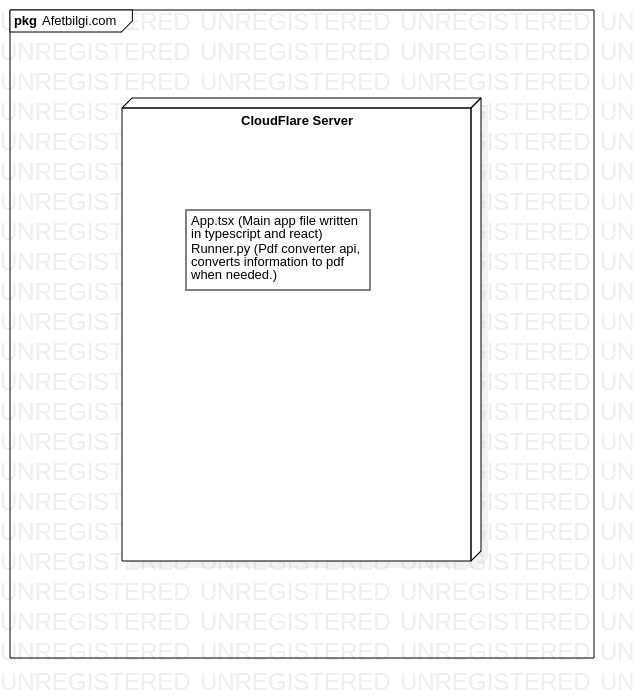
\includegraphics[scale = 0.5]{assets/DeploymentDiagram1.png}
    \caption[Deployment Diagram]{Deployment Diagram}
\end{figure}

\section{Design Rationale}

\begin{itemize}
    \item Application serves as a bridge between victims and volunteers.
    \item Systems setted up considering communication helps to improve viablity of information and speed of communication.
    %Functional view da iletişim halinde kurulan sistemlerle verinin doğruluğu ve ulaşım hızı sağlanıyor
    \item Database should be kept with MySQL and operations of database should be handled with MySQL node.js bridge.
    \item A statical version of website and pdfs should be kept and deployed in cloudflare servers for speeding up website.
\end{itemize}